\documentclass{standalone}
\usepackage{tikz}

\begin{document}
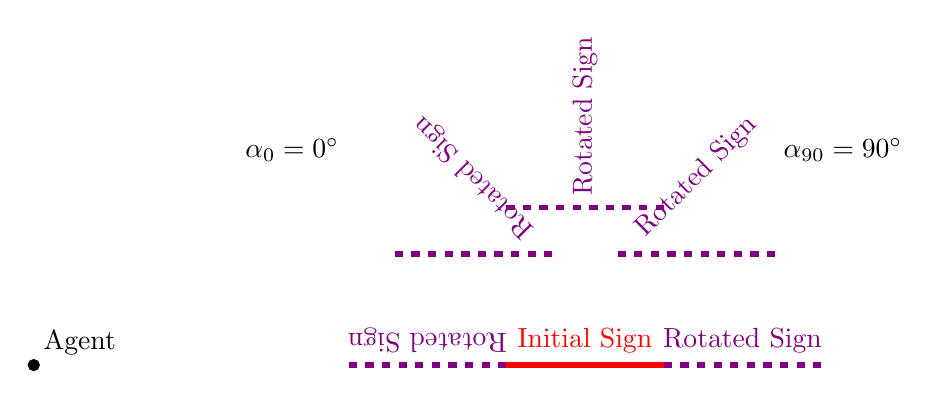
\begin{tikzpicture}[scale=2]

% Define coordinates for the agent cell (viewer)
\coordinate (agent) at (0, 0);

% Draw the agent cell (viewer) as a small circle
\filldraw[black] (agent) circle (1pt) node[above right] {Agent};

% Define the initial position of the exit sign
\coordinate (sign_initial) at (3, 0);

% Draw the exit sign initially aligned with the z-axis
\draw[line width=2pt, red] (sign_initial) -- ++(1,0) node[midway, above] {Initial Sign};

% Function to rotate the sign around the z-axis
\foreach \alpha in {0, 45, 90, 135, 180} {
    % Calculate new position after rotation
    \pgfmathsetmacro{\xnew}{3 + cos(\alpha)}
    \pgfmathsetmacro{\ynew}{sin(\alpha)}
    
    % Draw rotated sign
    \draw[line width=2pt, blue!50!red, dashed] (\xnew, \ynew) -- ++(1,0) node[midway, above] {\rotatebox{\alpha}{Rotated Sign}};
}

% Label the angles
\node at (2, 1.5) [below left] {$\alpha_0 = 0^\circ$};
\node at (4.7, 1.5) [below right] {$\alpha_{90} = 90^\circ$};

\end{tikzpicture}
\end{document}